% ============================================================
% Question Bank: ch05-03 Solving Equations with the Distributive Property
% Topic Title: Solving Equations with the Distributive Property
% CCSS: 7.EE.B.4a
% Questions: 27 (15 MC + 6 SA + 6 Graphical)
% ============================================================

% --- Multiple Choice Questions (15) ---

\begin{practiceQuestion}{5-3-q01}{mc}
\begin{questionText}
Solve $3(x + 5) = 33$.
\end{questionText}
\choiceA{$x = 6$}
\choiceB{$x = 9\frac{1}{3}$}
\choiceC{$x = 12$}
\choiceD{$x = 16$}
\correctAnswer{A}
\explanation{Divide both sides by $3$: $x + 5 = 11$. Subtract $5$: $x = 6$. Check: $3(6 + 5) = 3(11) = 33$ \checkmark.}
\end{practiceQuestion}

\begin{practiceQuestion}{5-3-q02}{mc}
\begin{questionText}
Solve $4(n - 7) = -12$.
\end{questionText}
\choiceA{$n = 4$}
\choiceB{$n = -10$}
\choiceC{$n = 10$}
\choiceD{$n = -4$}
\correctAnswer{A}
\explanation{Divide by $4$: $n - 7 = -3$. Add $7$: $n = 4$. Check: $4(4 - 7) = 4(-3) = -12$ \checkmark.}
\end{practiceQuestion}

\begin{practiceQuestion}{5-3-q03}{mc}
\begin{questionText}
Which equation is equivalent to $5(x + 3) = 40$?
\end{questionText}
\choiceA{$5x + 3 = 40$}
\choiceB{$5x + 15 = 40$}
\choiceC{$x + 15 = 40$}
\choiceD{$5x + 8 = 40$}
\correctAnswer{B}
\explanation{Distribute $5$: $5 \times x + 5 \times 3 = 5x + 15$. So the equation becomes $5x + 15 = 40$.}
\end{practiceQuestion}

\begin{practiceQuestion}{5-3-q04}{mc}
\begin{questionText}
Solve $-6(y + 2) = 30$.
\end{questionText}
\choiceA{$y = -7$}
\choiceB{$y = 3$}
\choiceC{$y = -3$}
\choiceD{$y = 7$}
\correctAnswer{A}
\explanation{Divide by $-6$: $y + 2 = -5$. Subtract $2$: $y = -7$. Check: $-6(-7 + 2) = -6(-5) = 30$ \checkmark.}
\end{practiceQuestion}

\begin{practiceQuestion}{5-3-q05}{mc}
\begin{questionText}
Solve $8(x - 3) = 0$.
\end{questionText}
\choiceA{$x = 0$}
\choiceB{$x = -3$}
\choiceC{$x = 3$}
\choiceD{$x = 8$}
\correctAnswer{C}
\explanation{Divide by $8$: $x - 3 = 0$. Add $3$: $x = 3$. Check: $8(3 - 3) = 8(0) = 0$ \checkmark.}
\end{practiceQuestion}

\begin{practiceQuestion}{5-3-q06}{mc}
\begin{questionText}
A student solved $4(x + 6) = 48$ and wrote: $4x + 6 = 48$, $4x = 42$, $x = 10.5$. What error did the student make?
\end{questionText}
\choiceA{Subtracted $6$ from the wrong side}
\choiceB{Did not distribute $4$ to the $6$}
\choiceC{Divided by $4$ instead of subtracting}
\choiceD{Added $6$ instead of subtracting}
\correctAnswer{B}
\explanation{The student wrote $4x + 6$ instead of $4x + 24$. Distributing correctly gives $4x + 24 = 48$, so $x = 6$.}
\end{practiceQuestion}

\begin{practiceQuestion}{5-3-q07}{mc}
\begin{questionText}
Solve $2(5x + 3) = 46$.
\end{questionText}
\choiceA{$x = 4$}
\choiceB{$x = 8$}
\choiceC{$x = 5$}
\choiceD{$x = 2$}
\correctAnswer{A}
\explanation{Distribute: $10x + 6 = 46$. Subtract $6$: $10x = 40$. Divide by $10$: $x = 4$. Check: $2(5(4) + 3) = 2(23) = 46$ \checkmark.}
\end{practiceQuestion}

\begin{practiceQuestion}{5-3-q08}{mc}
\begin{questionText}
Solve $-3(2x - 4) = 30$.
\end{questionText}
\choiceA{$x = -3$}
\choiceB{$x = 3$}
\choiceC{$x = 7$}
\choiceD{$x = -7$}
\correctAnswer{A}
\explanation{Distribute: $-6x + 12 = 30$. Subtract $12$: $-6x = 18$. Divide by $-6$: $x = -3$. Check: $-3(2(-3) - 4) = -3(-10) = 30$ \checkmark.}
\end{practiceQuestion}

\begin{practiceQuestion}{5-3-q09}{mc}
\begin{questionText}
What is the first step to solve $9(x + 1) = 63$ using the ``divide first'' method?
\end{questionText}
\choiceA{Subtract $1$ from both sides}
\choiceB{Distribute $9$ to get $9x + 9 = 63$}
\choiceC{Divide both sides by $9$}
\choiceD{Subtract $9$ from both sides}
\correctAnswer{C}
\explanation{The ``divide first'' method divides both sides by $9$: $x + 1 = 7$.}
\end{practiceQuestion}

\begin{practiceQuestion}{5-3-q10}{mc}
\begin{questionText}
Each side of a regular pentagon is $(x + 2)$ cm. The perimeter is $45$ cm. What is $x$?
\end{questionText}
\choiceA{$x = 7$}
\choiceB{$x = 9$}
\choiceC{$x = 43$}
\choiceD{$x = 11$}
\correctAnswer{A}
\explanation{Perimeter $= 5(x + 2) = 45$. Divide by $5$: $x + 2 = 9$. Subtract $2$: $x = 7$.}
\end{practiceQuestion}

\begin{practiceQuestion}{5-3-q11}{mc}
\begin{questionText}
Solve $-7(x + 1) = -35$.
\end{questionText}
\choiceA{$x = -6$}
\choiceB{$x = 4$}
\choiceC{$x = 6$}
\choiceD{$x = -4$}
\correctAnswer{B}
\explanation{Divide by $-7$: $x + 1 = 5$. Subtract $1$: $x = 4$. Check: $-7(4 + 1) = -7(5) = -35$ \checkmark.}
\end{practiceQuestion}

\begin{practiceQuestion}{5-3-q12}{mc}
\begin{questionText}
Solve $3(4x - 2) = 54$.
\end{questionText}
\choiceA{$x = 4$}
\choiceB{$x = 5$}
\choiceC{$x = 6$}
\choiceD{$x = 4\frac{2}{3}$}
\correctAnswer{B}
\explanation{Distribute: $12x - 6 = 54$. Add $6$: $12x = 60$. Divide by $12$: $x = 5$. Check: $3(4(5) - 2) = 3(18) = 54$ \checkmark.}
\end{practiceQuestion}

\begin{practiceQuestion}{5-3-q13}{mc}
\begin{questionText}
Four friends share the cost of a birthday present equally. Each person also pays $\$6$ for a card. Each person's total is $\$21$. What is the cost $c$ of the present?
\end{questionText}
\choiceA{$c = 84$}
\choiceB{$c = 60$}
\choiceC{$c = 15$}
\choiceD{$c = 108$}
\correctAnswer{B}
\explanation{Each pays $\frac{c}{4} + 6 = 21$. Subtract $6$: $\frac{c}{4} = 15$. Multiply by $4$: $c = 60$.}
\end{practiceQuestion}

\begin{practiceQuestion}{5-3-q14}{mc}
\begin{questionText}
Solve $12(x + 5) = 84$.
\end{questionText}
\choiceA{$x = 2$}
\choiceB{$x = 7$}
\choiceC{$x = 12$}
\choiceD{$x = \dfrac{29}{12}$}
\correctAnswer{A}
\explanation{Divide by $12$: $x + 5 = 7$. Subtract $5$: $x = 2$. Check: $12(2 + 5) = 12(7) = 84$ \checkmark.}
\end{practiceQuestion}

\begin{practiceQuestion}{5-3-q15}{mc}
\begin{questionText}
Solve $-4(3n + 5) = -32$.
\end{questionText}
\choiceA{$n = 1$}
\choiceB{$n = -1$}
\choiceC{$n = 3$}
\choiceD{$n = -3$}
\correctAnswer{A}
\explanation{Divide by $-4$: $3n + 5 = 8$. Subtract $5$: $3n = 3$. Divide by $3$: $n = 1$. Check: $-4(3(1) + 5) = -4(8) = -32$ \checkmark.}
\end{practiceQuestion}

% --- Short Answer Questions (6) ---

\begin{practiceQuestion}{5-3-q16}{sa}
\begin{questionText}
Solve $6(x + 4) = 42$.
\end{questionText}
\correctAnswer{$x = 3$}
\explanation{Divide by $6$: $x + 4 = 7$. Subtract $4$: $x = 3$. Check: $6(3 + 4) = 6(7) = 42$ \checkmark.}
\end{practiceQuestion}

\begin{practiceQuestion}{5-3-q17}{sa}
\begin{questionText}
Solve $-5(n - 6) = 40$.
\end{questionText}
\correctAnswer{$n = -2$}
\explanation{Divide by $-5$: $n - 6 = -8$. Add $6$: $n = -2$. Check: $-5(-2 - 6) = -5(-8) = 40$ \checkmark.}
\end{practiceQuestion}

\begin{practiceQuestion}{5-3-q18}{sa}
\begin{questionText}
Solve $7(2x + 3) = 77$.
\end{questionText}
\correctAnswer{$x = 4$}
\explanation{Divide by $7$: $2x + 3 = 11$. Subtract $3$: $2x = 8$. Divide by $2$: $x = 4$. Check: $7(2(4) + 3) = 7(11) = 77$ \checkmark.}
\end{practiceQuestion}

\begin{practiceQuestion}{5-3-q19}{sa}
\begin{questionText}
Solve $2(x - 9) = -10$.
\end{questionText}
\correctAnswer{$x = 4$}
\explanation{Divide by $2$: $x - 9 = -5$. Add $9$: $x = 4$. Check: $2(4 - 9) = 2(-5) = -10$ \checkmark.}
\end{practiceQuestion}

\begin{practiceQuestion}{5-3-q20}{sa}
\begin{questionText}
Each side of a regular hexagon is $(2x - 1)$ cm. The perimeter is $54$ cm. Find $x$.
\end{questionText}
\correctAnswer{$x = 5$}
\explanation{$6(2x - 1) = 54$. Divide by $6$: $2x - 1 = 9$. Add $1$: $2x = 10$. Divide by $2$: $x = 5$. Each side is $9$ cm.}
\end{practiceQuestion}

\begin{practiceQuestion}{5-3-q21}{sa}
\begin{questionText}
Solve $-10(x + 3) = 20$.
\end{questionText}
\correctAnswer{$x = -5$}
\explanation{Divide by $-10$: $x + 3 = -2$. Subtract $3$: $x = -5$. Check: $-10(-5 + 3) = -10(-2) = 20$ \checkmark.}
\end{practiceQuestion}

% --- Graphical MC Questions (3) ---

\begin{practiceQuestion}{5-3-q22}{gmc}
\begin{questionText}
The rectangle below has an area of $72$ square cm. What is the value of $x$?

\begin{center}
\begin{tikzpicture}[scale=0.6]
  \draw[thick,fill=funBlue!10] (0,0) rectangle (8,3);
  \draw[<->] (0,-0.5) -- (8,-0.5);
  \node[below] at (4,-0.5) {$8$ cm};
  \draw[<->] (-0.5,0) -- (-0.5,3);
  \node[left] at (-0.5,1.5) {$(x + 4)$ cm};
\end{tikzpicture}
\end{center}
\end{questionText}
\choiceA{$x = 5$}
\choiceB{$x = 9$}
\choiceC{$x = 13$}
\choiceD{$x = 4$}
\correctAnswer{A}
\explanation{Area $= 8(x + 4) = 72$. Divide by $8$: $x + 4 = 9$. Subtract $4$: $x = 5$.}
\end{practiceQuestion}

\begin{practiceQuestion}{5-3-q23}{gmc}
\begin{questionText}
The triangle below has a perimeter of $36$ inches. Each side has the same length. What is $x$?

\begin{center}
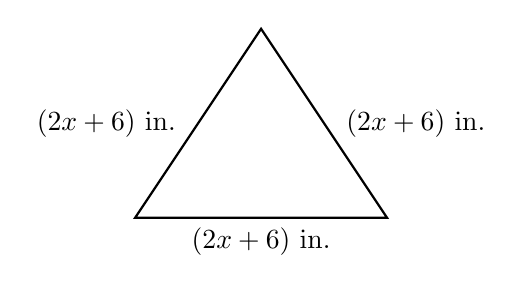
\begin{tikzpicture}[scale=0.8]
  \draw[thick] (0,0) -- (4,0) -- (2,3) -- cycle;
  \node[below] at (2,0) {$(2x + 6)$ in.};
  \node[right] at (3.2,1.5) {$(2x + 6)$ in.};
  \node[left] at (0.8,1.5) {$(2x + 6)$ in.};
\end{tikzpicture}
\end{center}
\end{questionText}
\choiceA{$x = 3$}
\choiceB{$x = 5$}
\choiceC{$x = 6$}
\choiceD{$x = 9$}
\correctAnswer{A}
\explanation{Perimeter $= 3(2x + 6) = 36$. Divide by $3$: $2x + 6 = 12$. Subtract $6$: $2x = 6$. Divide by $2$: $x = 3$.}
\end{practiceQuestion}

\begin{practiceQuestion}{5-3-q24}{gmc}
\begin{questionText}
The balance scale below is in equilibrium. What is $x$?

\begin{center}
\begin{tikzpicture}[scale=0.7]
  % Fulcrum
  \draw[thick] (0,-0.5) -- (-0.4,-1.2) -- (0.4,-1.2) -- cycle;
  % Beam
  \draw[thick] (-4.5,0) -- (4.5,0);
  % Left pan: 2 groups of (x+4)
  \draw[thick] (-4,0) -- (-4.8,-0.6) -- (-3.2,-0.6) -- (-4,0);
  \draw[thick,fill=funBlue!20] (-4.8,-0.6) -- (-4.8,-1) -- (-3.2,-1) -- (-3.2,-0.6) -- cycle;
  \node at (-4,-0.8) {\small $2(x + 4)$};
  % Right pan
  \draw[thick] (4,0) -- (4.8,-0.6) -- (3.2,-0.6) -- (4,0);
  \draw[thick,fill=funOrange!20] (4.8,-0.6) -- (4.8,-1) -- (3.2,-1) -- (3.2,-0.6) -- cycle;
  \node at (4,-0.8) {\small $26$};
\end{tikzpicture}
\end{center}
\end{questionText}
\choiceA{$x = 7$}
\choiceB{$x = 9$}
\choiceC{$x = 11$}
\choiceD{$x = 13$}
\correctAnswer{B}
\explanation{The balance gives $2(x + 4) = 26$. Divide by $2$: $x + 4 = 13$. Subtract $4$: $x = 9$.}
\end{practiceQuestion}

% --- Graphical SA Questions (3) ---

\begin{practiceQuestion}{5-3-q25}{gsa}
\begin{questionText}
The large rectangle is divided into $5$ equal smaller rectangles, each with a width of $(x - 2)$ cm. The total area of the large rectangle is $100$ cm$^{2}$ and its height is $4$ cm. Find $x$.

\begin{center}
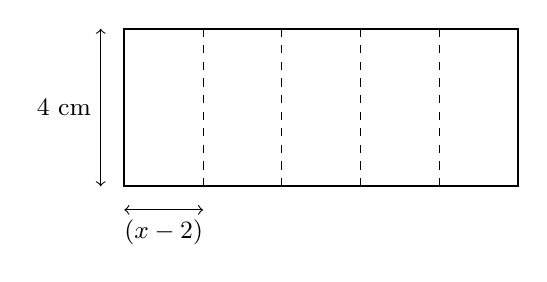
\begin{tikzpicture}[scale=0.5]
  \draw[thick] (0,0) rectangle (10,4);
  \foreach \i in {2,4,6,8} \draw[dashed] (\i,0) -- (\i,4);
  \draw[<->] (0,-0.6) -- (2,-0.6);
  \node[below] at (1,-0.6) {\small $(x-2)$};
  \draw[<->] (-0.6,0) -- (-0.6,4);
  \node[left] at (-0.6,2) {\small $4$ cm};
\end{tikzpicture}
\end{center}
\end{questionText}
\correctAnswer{$x = 7$}
\explanation{Total width $= 5(x - 2)$. Area $= 4 \times 5(x - 2) = 100$. Divide by $4$: $5(x - 2) = 25$. Divide by $5$: $x - 2 = 5$. Add $2$: $x = 7$.}
\end{practiceQuestion}

\begin{practiceQuestion}{5-3-q26}{gsa}
\begin{questionText}
A square garden has a side length of $(3x + 1)$ feet. Its perimeter is $76$ feet. Find $x$.

\begin{center}
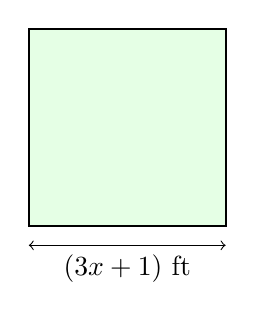
\begin{tikzpicture}[scale=0.5]
  \draw[thick,fill=green!10] (0,0) rectangle (5,5);
  \draw[<->] (0,-0.5) -- (5,-0.5);
  \node[below] at (2.5,-0.5) {$(3x + 1)$ ft};
\end{tikzpicture}
\end{center}
\end{questionText}
\correctAnswer{$x = 6$}
\explanation{Perimeter $= 4(3x + 1) = 76$. Divide by $4$: $3x + 1 = 19$. Subtract $1$: $3x = 18$. Divide by $3$: $x = 6$.}
\end{practiceQuestion}

\begin{practiceQuestion}{5-3-q27}{gsa}
\begin{questionText}
The balance scale below is in equilibrium. Find $n$.

\begin{center}
\begin{tikzpicture}[scale=0.7]
  % Fulcrum
  \draw[thick] (0,-0.5) -- (-0.4,-1.2) -- (0.4,-1.2) -- cycle;
  % Beam
  \draw[thick] (-4.5,0) -- (4.5,0);
  % Left pan
  \draw[thick] (-4,0) -- (-4.8,-0.6) -- (-3.2,-0.6) -- (-4,0);
  \draw[thick,fill=funBlue!20] (-4.8,-0.6) -- (-4.8,-1) -- (-3.2,-1) -- (-3.2,-0.6) -- cycle;
  \node at (-4,-0.8) {\small $5(n + 3)$};
  % Right pan
  \draw[thick] (4,0) -- (4.8,-0.6) -- (3.2,-0.6) -- (4,0);
  \draw[thick,fill=funOrange!20] (4.8,-0.6) -- (4.8,-1) -- (3.2,-1) -- (3.2,-0.6) -- cycle;
  \node at (4,-0.8) {\small $60$};
\end{tikzpicture}
\end{center}
\end{questionText}
\correctAnswer{$n = 9$}
\explanation{The balance gives $5(n + 3) = 60$. Divide by $5$: $n + 3 = 12$. Subtract $3$: $n = 9$. Check: $5(9 + 3) = 5(12) = 60$ \checkmark.}
\end{practiceQuestion}
